\documentclass[notitlepage,11pt]{report}


% Packages
% --------
%	 Necessary
\usepackage{geometry} 						% geometry - page dimensions
\usepackage[parfill]{parskip}				% parskip - to use blank line to sep paragraphs
\usepackage{titling}						% title formatting
\usepackage{enumitem}

\usepackage{amsmath}						% AMS - math, fonts, symbols, theorem
\usepackage{amsfonts}
\usepackage{amssymb}
\usepackage{amsthm}
\usepackage{mathtools}						% mathtools - \coloneqq

\usepackage{listings}						% listings - prints source code

\usepackage{hyperref}						% hyperref - urls and things

\usepackage{tikz}							% tikz - graphs

% 	Additional
\usepackage{graphicx}						% graphicx - importing graphics from file
\usepackage{subcaption}
\captionsetup[subfigure]{labelformat=empty}
\usepackage[T1]{fontenc}
\usepackage[utf8]{inputenc}
\usepackage{helvet}
\renewcommand{\familydefault}{\sfdefault}	% change to helvetica

\usepackage{forest}							% forest - easy trees
\usepackage{tikzsymbols}					% tikzsymbols - just adds some symbols
% tikzlibrary summary: 
% tex.stackexchange.com/questions/42611/list-of-available-tikz-libraries-with-a-short-introduction/491626
\usetikzlibrary{arrows.meta}				% arrows.meta - customizable arrow tips
\usetikzlibrary{er}							% entity-relationship diagrams
\usetikzlibrary{positioning} 				% relative positioning
\usetikzlibrary{shadows}
\usetikzlibrary{shapes}

\usepackage{xcolor}							% xcolor - adds additional colors

\usepackage{marginnote}						% marginnote - see name

\usepackage{multirow}						% multirow - sort of a tabular environment of text
\usepackage{bigdelim}						% bigdelim - used with multirow once to make brackets on tables
\usepackage{array}							% array - extends arrary and tabular environment
\usepackage{makecell}						% makecell - adjust cell cizes within tabular environment

\usepackage[bottom]{footmisc}				% comment out to make footnotes not appear at bottom of page

% Customizations

\pretitle{\begin{center}\Large\bfseries}		% titling format
\posttitle{\par\end{center}\vskip 0cm}
\preauthor{\begin{center}\large}
\postauthor{\end{center}}
\predate{\par\normalsize\centering}
\postdate{\par}

\newtheoremstyle{customnumber} % name
	{}% space above
	{}% space below
	{\normalfont}% body font
	{}% indent 
	{\bfseries}% head font
	{:}% punctuation between head/body
	{ }% space after head: " " = normal whitespace
	{\thmname{#1}\thmnote{ #3}}% head format

\newtheoremstyle{named}
	{}
	{}
	{\normalfont}
	{}
	{\bfseries}
	{.}
	{ }
	{\thmnote{#3}}

\theoremstyle{customnumber}
\newtheorem*{exercise}{Exercise}

\theoremstyle{definition}
\newtheorem{defi}{Definition}

\newtheorem{ex}{Example}[section]

\theoremstyle{named}
\newtheorem*{namedtheorem}{}

\newenvironment{absolutelynopagebreak}
	{\par\nobreak\vfil\penalty0\vfilneg\vtop\bgroup}
	{\par\xdef\tpd{\the\prevdepth}\egroup\prevdepth=\tpd}
	
\newcommand{\indep}{\raisebox{0.05em}{\rotatebox[origin=c]{90}{$\models$}}}

\newcommand{\stcomp}[1]{{#1}^\complement}


\lstset{tabsize=3, numbers=left, basicstyle=\ttfamily, escapeinside=~~, xleftmargin=-1cm}
\let\origthelstnumber\thelstnumber
\makeatletter
\newcommand*\Suppressnumber{%
	\lst@AddToHook{OnNewLine}{%
		\let\thelstnumber\relax%
		\advance\c@lstnumber-\@ne\relax%
	}%
}
\newcommand*\Reactivatenumber{%
	\lst@AddToHook{OnNewLine}{%
		\let\thelstnumber\origthelstnumber%
		\advance\c@lstnumber\@ne\relax%
	}%
}
\makeatother

\title{Activity 7}
\author{}
\date{}

\begin{document}
\maketitle
\begin{center} Entities: \end{center}
Products: barcode (ID), name, price, quantity, supplier)

Customers: name, address, customerid, phone, payment info, email

\begin{center} Relationships: \end{center}
Purchases: date, quantity, price, tax, total cost

\begin{center}
	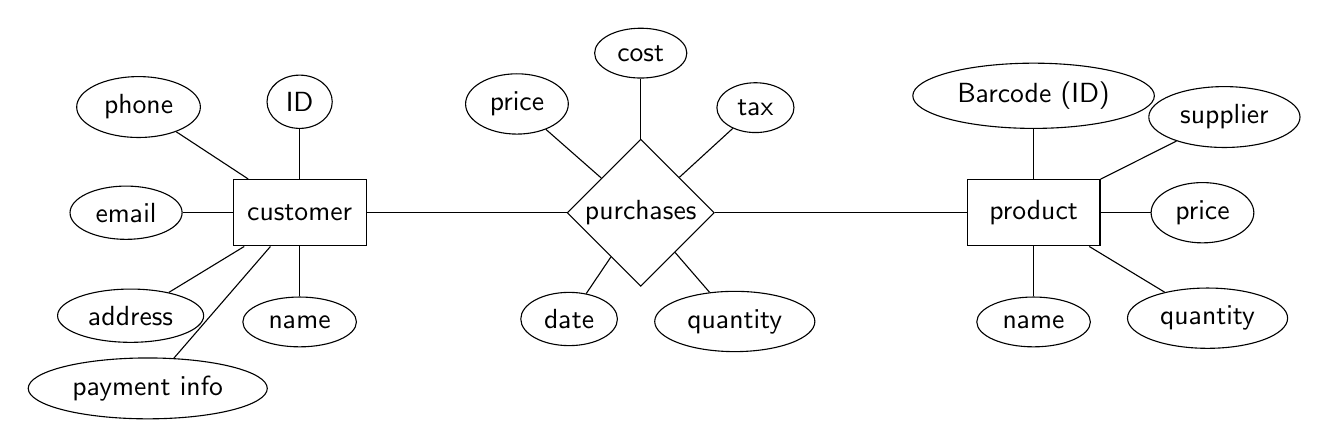
\begin{tikzpicture}
	\node[entity] (customer) {customer};
	\node[entity] (product) [right=3in of customer] {product};
	\node[relationship] (purchases) [right=1in of customer] {purchases}				edge (customer) edge (product);
%	\foreach \i in {-1, 1}{%
%	\draw[-] (customer.east) -- ([yshift=\i * 0.5 em]purchases.west); 
%	\draw[-] (product.west) -- ([yshift=\i * 0.5 em]purchases.east);
%	}
	\node[attribute] (customerID) [above=0.25in of customer] {ID}
	edge (customer);
	\node[attribute] (customerName) [below=0.25in of customer] {name}
	edge (customer);
	\node[attribute] (customerEmail) [left=0.25in of customer] {email}
	edge (customer);
	\node[attribute] (customerAddress) [below left=0.25in and 0.25in of customer] {address}
	edge (customer);
	\node[attribute] (customerPhone) [above left=0.25in and 0.25in of customer] {phone}
	edge (customer);
	\node[attribute] (customerPayInfo) [below left=0.6in and 0in of customer] {payment info}
	edge (customer);
	
	\node[attribute] (purchaseDate) [below left=0.25in and 0in of purchases] {date}
	edge (purchases);
	\node[attribute] (purchaseQuantity) [below right=0.25in and 0in of purchases] {quantity}
	edge (purchases);
	\node[attribute] (purchasePrice) [above left=0.25in and 0.25in of purchases] {price}
	edge (purchases);
	\node[attribute] (purchaseTax) [above right=0.25in and 0.25in of purchases] {tax}
	edge (purchases);
	\node[attribute] (purchaseCost) [above=0.3in of purchases] {cost}
	edge (purchases);
	
	\node[attribute] (productID) [above=0.25in of product] {Barcode (ID)}
	edge (product);
	\node[attribute] (productName) [below=0.25in of product] {name}
	edge (product);
	\node[attribute] (productPrice) [right=0.25in of product] {price}
	edge (product);
	\node[attribute] (productQuantity) [below right=0.25in and 0.25in of product] {quantity}
	edge (product);
	\node[attribute] (productSupplier) [above right=0.2in and 0.35in of product] {supplier}
	edge (product);
	\end{tikzpicture}
\end{center}

\end{document}